\section{Database design}
\begin{figure}[h!]
\centering
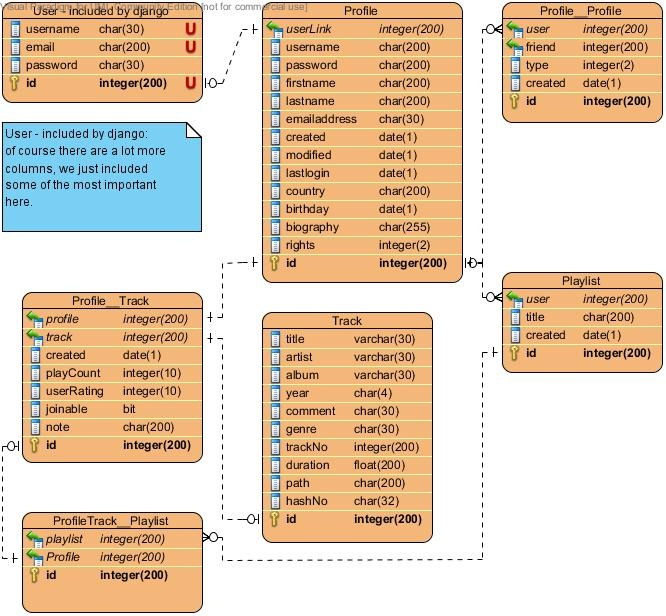
\includegraphics[scale=0.5]{design/figures/mwdbdiagram}
\caption{Movingwhales Database Diagram}
\end{figure}
The structure of the database is created by Django's ORM from the models written by the group. As it can be seen from the figure above, there
are 7 tables: Profile, User, Profile\_\_Profile, Playlist, Track, Profile\_\_Track and 
ProfileTrack\_\_Playlist. There are several other tables in the database, but these are never referenced in the code of the 
project, and are only managed by Django. For ease of reading only tables and columns referenced in the code are shown. The 
Profile\_\_Profile, Profile\_\_Track and ProfileTrack\_\_Playlist are relations between models.
\begin{itemize}
\item The Profile table includes the columns userlink, username, password, firstname, lastname, emailaddress, created, modified, lastlogin, country, birthday, biography, rights and an id.  The userlink is a one-to-one key to one entry in the User table, which is created first. The username, password and emailaddress are also included in the User table, which is native to Django, however this was not discovered until the database had already been created, and it would be far more work to remove the columns than to simply not use the ones in the Profile table. The e-mail column in the Profile table is used to store the publicly available e-mail address, where the User table's e-mail column is used to store the e-mail with which the profile is registered. This e-mail cannot be changed once saved. The columns firstname, lastname, country, birthday and biography are used to introduce the social aspect of the page, these can be customized to give other users information about the owner of the profile. 

Created, modified, and lastlogin are for administrational purposes, in the event of a profile being compromised this shows if anything has been changed in the profile. The ``rights'' column shows the profile's rights on the page, i.e. whether they are a regular user, a moderator or and admin. This is not implemented in the current state of the project. 

The id is given to all tables automatically by Django.

\item The Track table stores information about a given track and includes the columns title, artist, album, year, comment, genre, trackNo, duration, path, hashNo and an id. This information is mostly what can be retrieved from and ID3-tag on a track, however hashNo and path are introduced by the group: The hashNo to give a name to the file and make sure that there are only unique tracks in the database, and the path to specify where on the server the track is located. 

\item The Playlist table contains the columns user, title, created and an id. Seeing as a playlist in this system is merely an id that tracks can refer to, it doesn't contain any actual data about the songs in it. The user column contains a foreign key to an entry in the Profile table.

\item The Profile\_\_Profile relation keeps track of the social aspect of having friends. It contains two foreign keys to two entries in the Profile table called user and friend, a type of relation, which can be either a friend or a request or an ignored person, a date of creation, and and id.

\item The Profile\_\_Track relation keeps track of which songs are added to a given profile. It contains two foreign keys, one to an entry in the Profile table (user) and one to an entry in the Track table (track). It also contains the date created, a user rating, a count of how many times it has been played, a joinable setting and a note which is not yet implemented, and an id. 

\item The last relation is the ProfileTrack\_\_Playlist relation, which only contains two foreign keys and an id. The foreign keys are to an entry in the Profile and in the Playlist table. This relation links tracks and playlists together through the Profile\_\_Track table.
\end{itemize}